\documentclass[mathserif,serif,handout]{beamer}

\setbeamertemplate{navigation symbols}{}

\usepackage{xcolor}
\usepackage[T1]{fontenc}
\usepackage{lmodern}
\usefonttheme{professionalfonts}

\definecolor{purple}{RGB}{57,39,91}
\definecolor{lightpurple}{RGB}{223,221,232}
\definecolor{LightGray}{rgb}{0.90,0.90,0.90}

\setbeamercolor{title}{bg=purple, fg=white}
\setbeamercolor{titlelike}{bg=purple, fg=white}
\setbeamercolor{background canvas}{bg=white}
\setbeamercolor{item projected}{fg=purple}
\setbeamercolor{item}{fg=purple}
\setbeamercolor{caption name}{fg=purple}

% Explainframes:
\usepackage{ifthen}
\newboolean{isexplainframe}
\setboolean{isexplainframe}{false}
\mode<handout>{
  \newenvironment{explainframe}[1]{
    \setboolean{isexplainframe}{true}
    \addtocounter{framenumber}{-1}
    \setbeamertemplate{background}[grid][step=5mm,color=LightGray]
    \begin{frame}{Handout only: #1}%
    }{%
    \end{frame}%
  \setboolean{isexplainframe}{false}
  }
}

\mode<beamer>{
  \newenvironment{explainframe}[1]{
  }
}

\setbeamertemplate{footline}{%
  \leavevmode%
  \hbox{%
    \begin{beamercolorbox}[wd=.7\paperwidth,ht=2.25ex,dp=1ex,center]{}%
    \end{beamercolorbox}%
    \begin{beamercolorbox}[wd=.3\paperwidth,ht=2.25ex,dp=1ex,right]{slide number}%
      \insertframenumber{}\ifthenelse{\boolean{isexplainframe}}{E}{} / \inserttotalframenumber\hspace*{2ex}
  \end{beamercolorbox}}%
  \vskip0pt%
}

\title[Query Visualization] % (optional, only for long titles)
{Visualizing Physical Query Execution in a Relational Big Data Management System}
\subtitle{}
%\institute{CSE @ UW}
\author[Chu, moritz] % (optional, for multiple authors)
{Shumo Chu, Dominik Moritz}

\begin{document}

\begin{frame}
\titlepage

\end{frame}

\begin{frame}
  \frametitle{Objective}
  \begin{itemize}
  	\item 
  \end{itemize}
\end{frame}

\begin{frame}
  \frametitle{The Myria System}
  \begin{itemize}
  	\item Big Data management system developed in db group
  	\item Pipelined, parallel, distributed dataflow evaluation system
  	\item \textbf{Fragments}: trees of operators that are each executed on one thread in each worker
  	\item Fragment leaves and roots are typically I/O operators
    \item Push\--based between fragments, pull\--based inside fragments
  \end{itemize}
\end{frame}

\begin{frame}
  \frametitle{Myria Architecture}
  \begin{figure}
   \begin{center}
       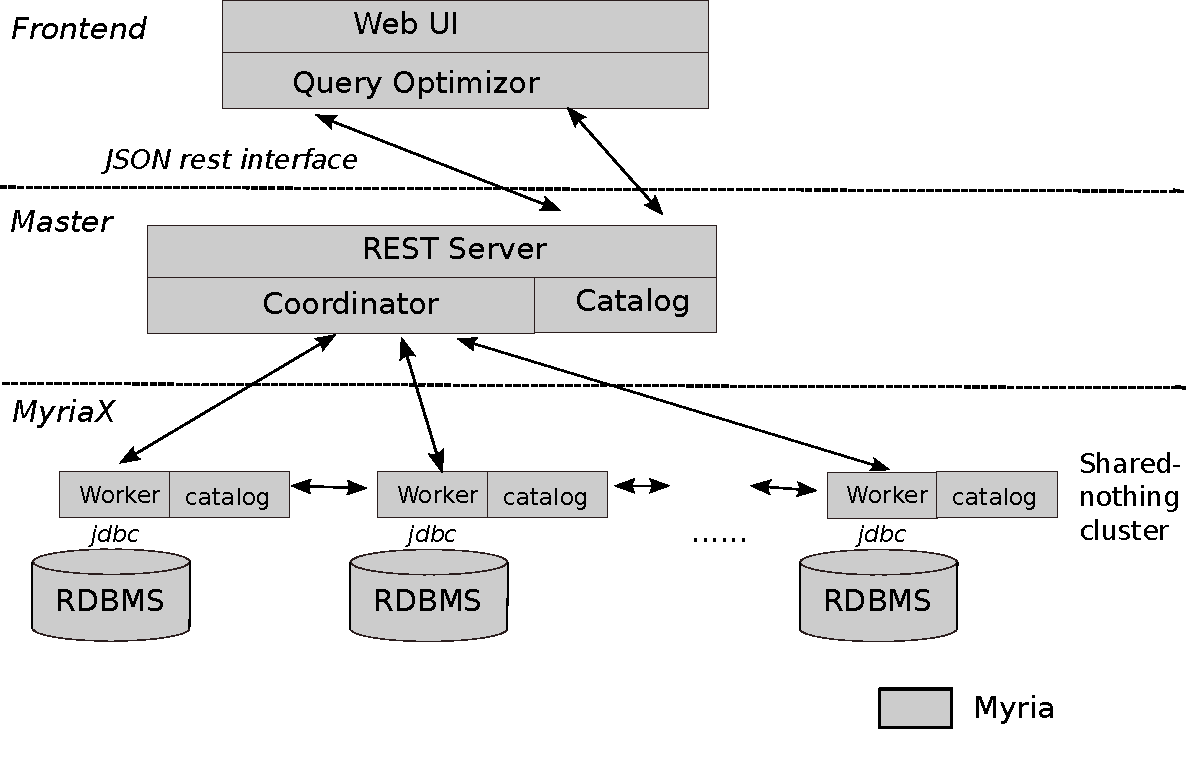
\includegraphics[width=0.9\textwidth]{myria_arch.pdf}
     \end{center}
    \caption{Myria System Architecture.}
    \label{fig:myria_arc}
  \end{figure}
\end{frame}

\begin{frame}{Physical query plan}
  \begin{figure}
   \begin{center}
       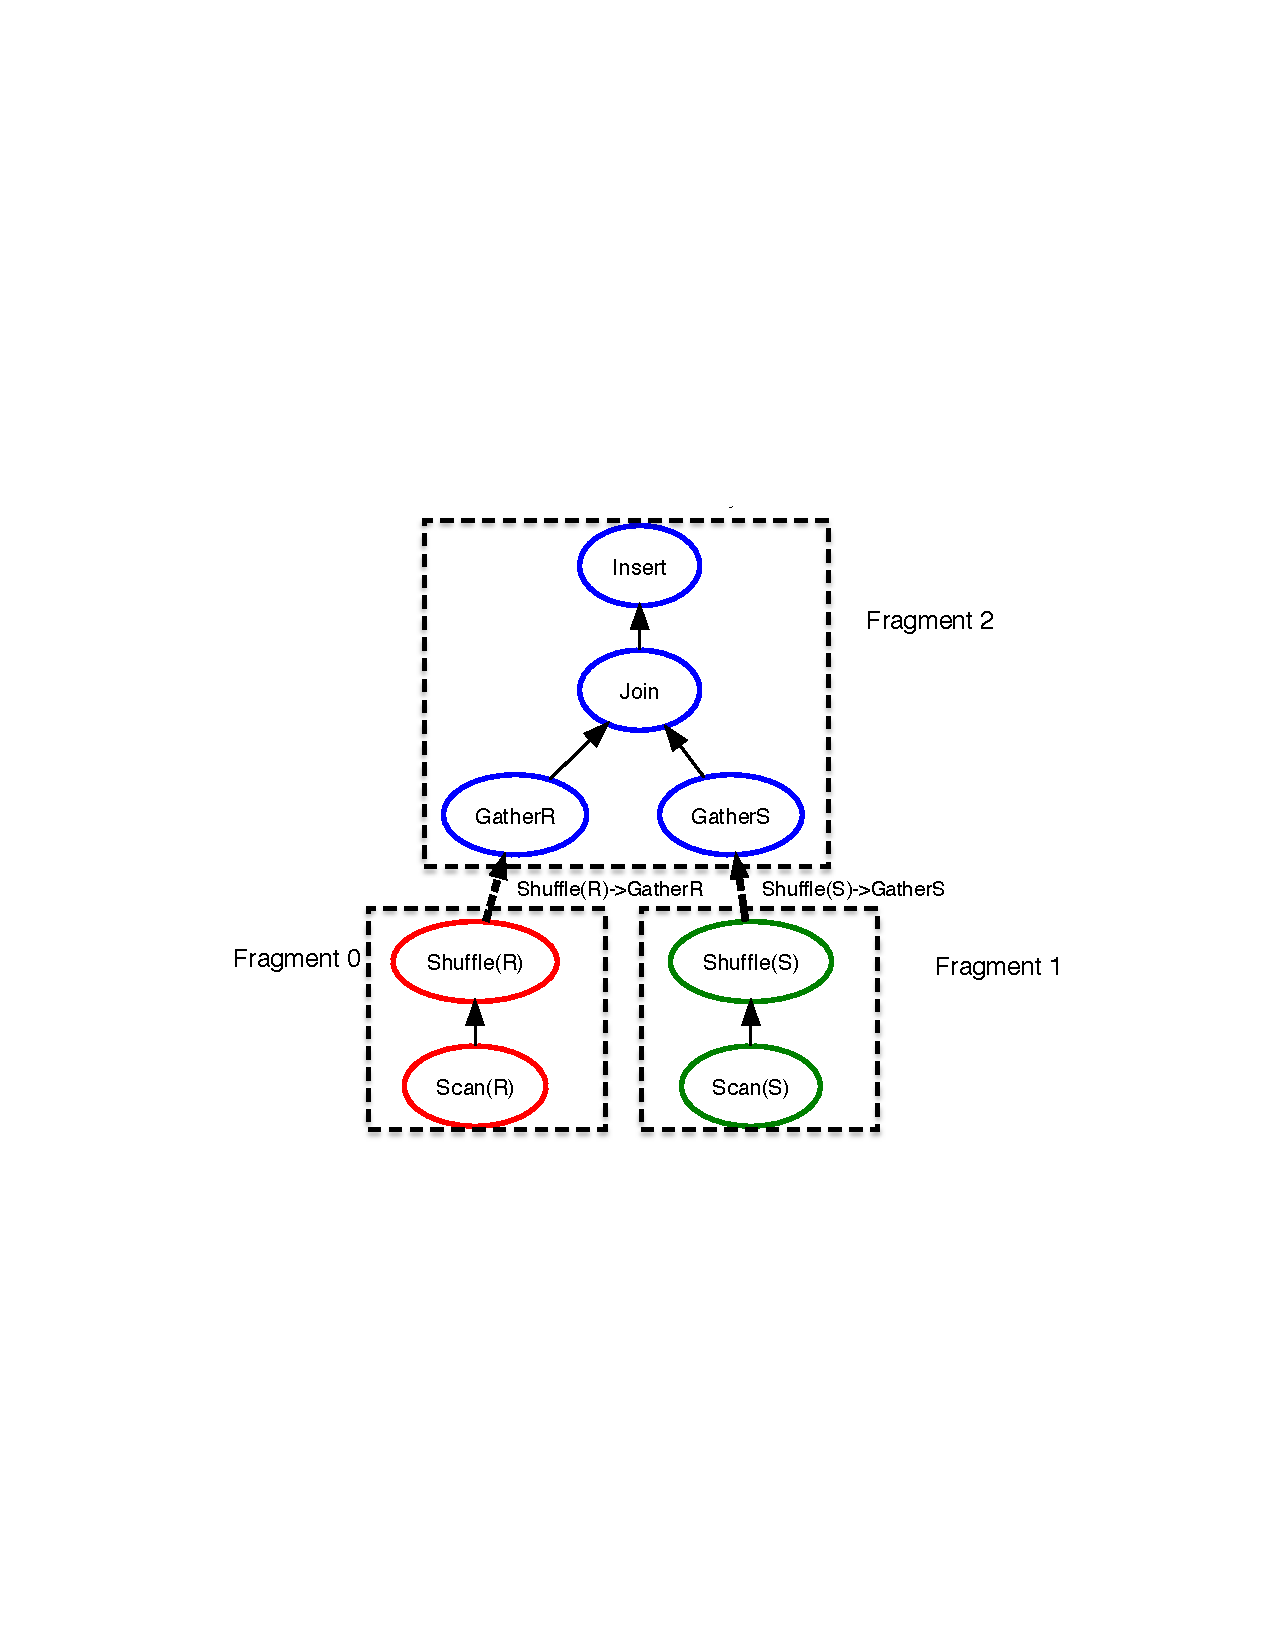
\includegraphics[width=.7\textwidth]{join}
     \end{center}
    \caption{Query plan of distributed hash join using three query fragments.}
  \end{figure}
\end{frame}

\begin{frame}
  \frametitle{Visualization}
  \begin{itemize}
    \item Three granularities
  \end{itemize}
  \begin{enumerate}
    \item Query level
    \begin{itemize}
      \item Shows utilization of workers
      \item Long tails indicate slow fragment
    \end{itemize}
    \item Fragment level
    \begin{itemize}
      \item Identify slow worker
      \item Utilization
      \item States of root operator on all worker over time
    \end{itemize}
    \item Operator level
    \begin{itemize}
      \item Identify low\--level problems
      \item Hierarchy of operators
      \item States per operator
    \end{itemize}
  \end{enumerate}
\end{frame}

\begin{explainframe}{Query plan level visualization}
  \begin{figure}
   \begin{center}
       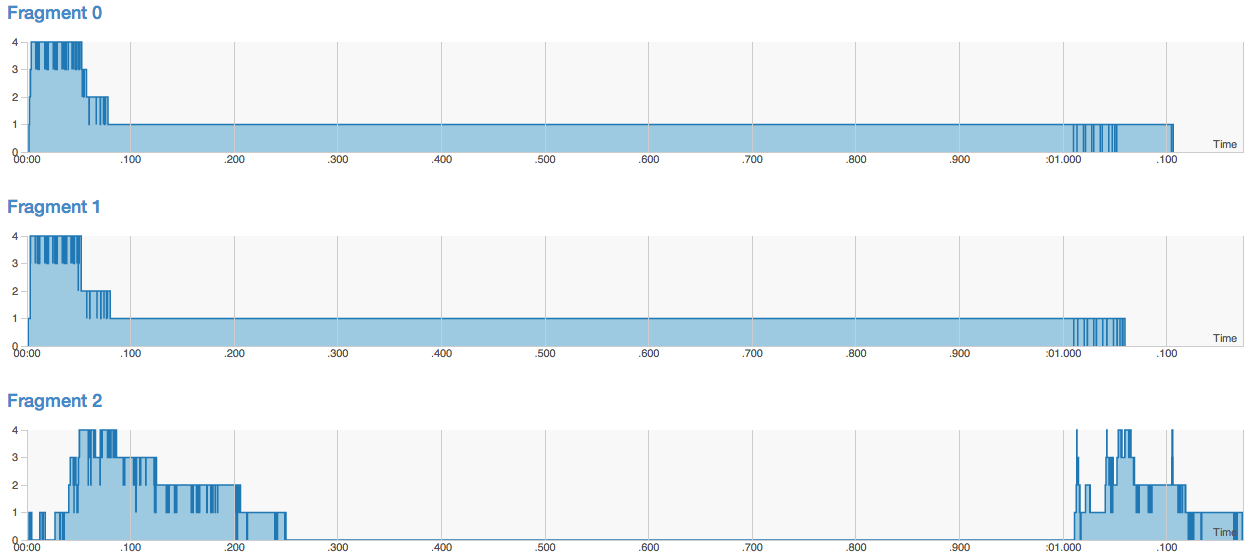
\includegraphics[width=\textwidth]{queryplanviz.png}
     \end{center}
    \caption{The \emph{query plan} visualization shows a line chart of cluster utilization for each fragment, measured as the fraction of workers executing it. In this view, a long tail identifies a query bottleneck.}
  \end{figure}
\end{explainframe}

\begin{explainframe}{Query fragment level visualization}
  \begin{figure}
   \begin{center}
       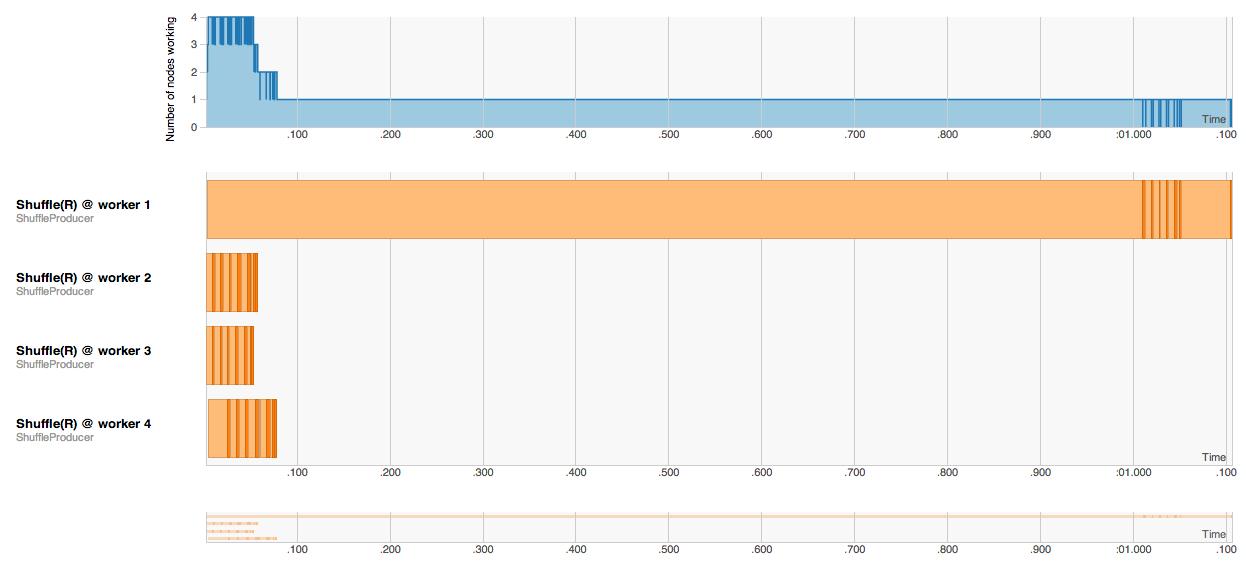
\includegraphics[width=\textwidth]{fragmentviz}
     \end{center}
    \caption{ By tracking the thread state across workers---\emph{computing}, \emph{sleeping}, \emph{sending}, or \emph{receiving}---users can identify performance anomalies and workload skew.}
  \end{figure}
\end{explainframe}

\begin{explainframe}{Operator level visualization}
  \begin{figure}
   \begin{center}
       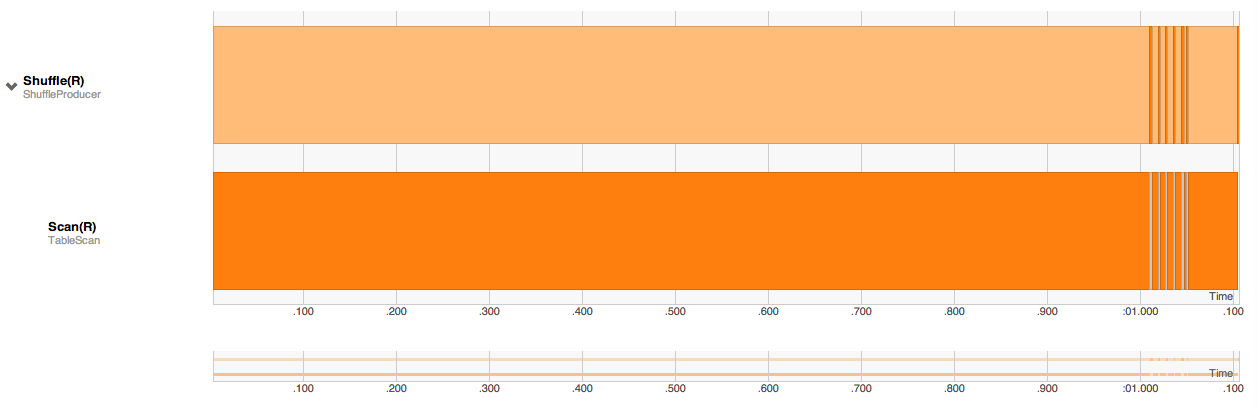
\includegraphics[width=\textwidth]{operatorviz}
     \end{center}
    \caption{The \emph{operator level} visualization shows a Gantt chart of operator states for a specific query fragment on a specific worker. The operators are shown in the same hierarchy as they appear in the query subtree. The fine-grained thread states are shown over time. This view allows users to identify or explain low-level implementation problems.}
  \end{figure}
\end{explainframe}

\begin{frame}
  \frametitle{Visualization: System Architecture}
  \begin{figure}
  	 \begin{center}
       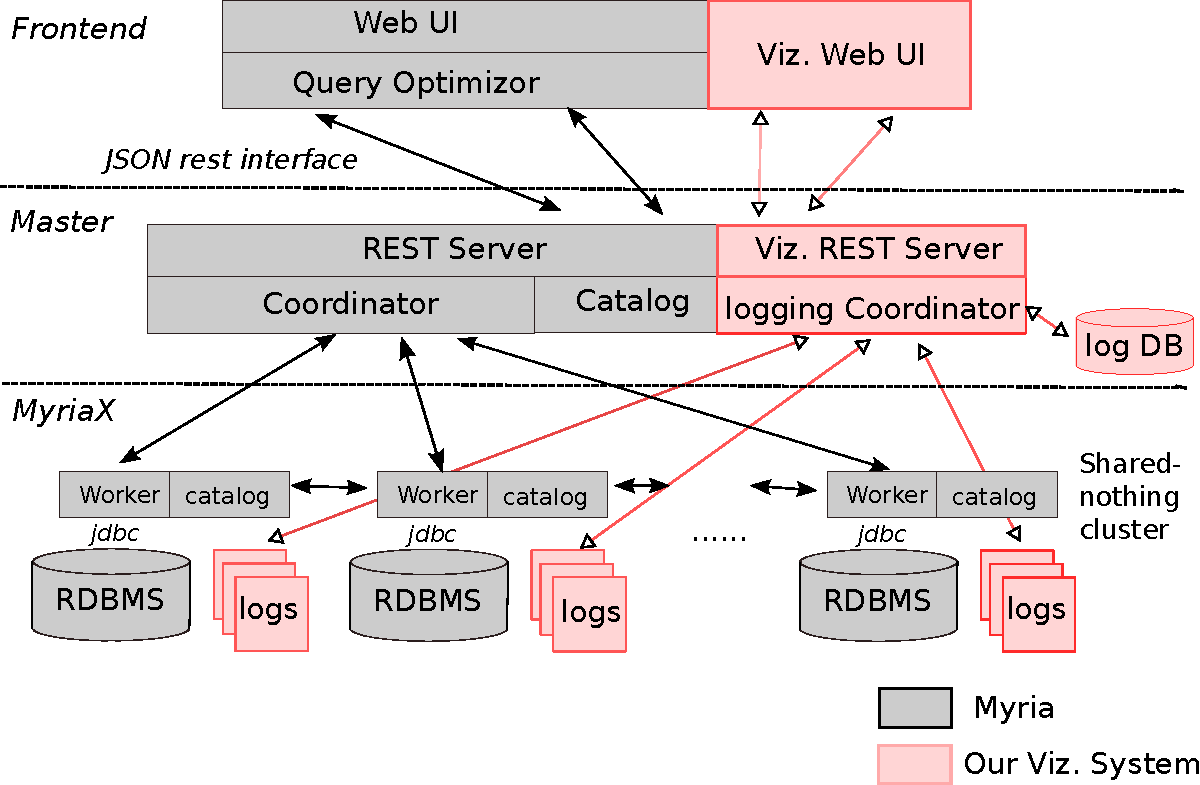
\includegraphics[width=0.9\textwidth]{viz_arch.pdf}
     \end{center}
     \caption{Visualization System Architecture.}
    \label{fig:viz_arc}
  \end{figure}
\end{frame}

\begin{frame}
  \frametitle{Demo}
\end{frame}

\end{document}